%-------------------------------------------------------------------------------
\chapter{Neurális hálózatok és a Deep Learning}
%-------------------------------------------------------------------------------
Ebben a fejezetben szeretném összegezni megszerzett tudásomat a neurális hálózatokról és a Deep Learning-ről, magyarul mély tanulásról. 
\section{A neurális hálózatok elmélete}
\label{section:neuralNetworkTheory}
% TODO ezt a bekezdést még dolgozd át!
%Olyan számítási modellel, amelynek alapját az idegrendszer hálózata adja először  Warren McCulloch és Walter Pitts 1943-ban foglalkozott az ,,A Logical Calculus of the Ideas Immanent in Nervous Activity'' című publikációjukban. Később Donald Hebb tanulással kapcsolatos megfigyeléseivel elindultak a mesterséges neurális hálókkal kapcsolatos kísérletezések.\cite{neural2006}

A mesterséges neurális hálózatok egy viszonylag egyszerű modellen alapulnak. Minden neuron a hozzá kapcsolódó neuronok ingereinek összessége alapján ingerli a többi neuront melyekhez ő kapcsolódik, ekképpen az ingerület egy irányba halad a kapcsolatok mentén.

Hogy a hálózat áttekinthető legyen, rendezzük a neuronokat rétegekbe úgy, hogy egy réteg neuronjai az ingerületet a közvetlen felső réteg neuronjaitól kapja, és a válasz ingert a közvetlenül alatta lévő réteg neuronjainak továbbítja.
\begin{figure}
	\centering
%	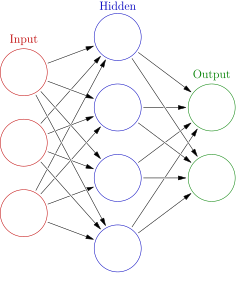
\includegraphics[width=0.9\textwidth]{Colored_neural_network.svg}
	\def\svgwidth{0.5\columnwidth}
	\input{fig/Colored_neural_network.pdf_tex}
	\caption{neurális hálózat réteges szerkezete \protect \footnotemark}
	\label{fig:neuralNet}
\end{figure}
\footnotetext{forrás: https://en.wikipedia.org/wiki/Artificial\_neural\_network}
A \ref{fig:neuralNet} ábrán a csúcsok jelentik a neuronokat és az élek a szinapszisok, melyeken az ingerület vándorol. Egy hálózat 3 nagyobb részre tagolódik:
\begin{enumerate*}[label={\alph*)},font=\bfseries]
	\item bemeneti réteg
	\item rejtett rétegek
	\item kimeneti réteg.
\end{enumerate*}
A bemeneti réteg csúcsai legtöbbször az adatot reprezentáló konstansok jelentik, tehát az egy egyszerű vektor.
Egy neuronban két művelet történik: a bementek összegzése és egy aktiváló függvény kiértékelés. Az összegzést a felsőbb rétegből érkező jelekre elvégezzük:
\begin{equation}
	s = \sum_i{w_ix_i} = \vec{w}\cdot\vec{x}
\end{equation}
ahol $x_i$ a felső réteg i.-ik neuronjának kimenete, $w_i$ az i.-ik neuron szinapszisához tartozó súly, mellyel a szinapszis "erősségét" határozzuk meg. Az "s" összeghez hozzáadunk még egy $b$ értéket, a neuron aktiválási küszöbértéke lesz.
Az aktivációs függvény adja a neurális hálózat kimenetét, paramétere $s+b$.
A neurális hálózatok fejlesztésekor sokféle függvényt találtak alkalmasnak aktivációs függvény gyanánt. Közös jellemzőjük, hogy inflexiós pontjuk $x=0$ helyen van, illetve 0-ban nem deriválható függvények esetén a töréspont esik ide. Leggyakoribbak talán az egységugrás, a $\tanh(x)$, az ún. ReLU vagyis a $\max\{0,x\}$, szigmoid ($\sigma(x)= \frac{1}{1+e^{-x}}$) és a \emph{softmax} függvények. Utóbbi kettőt az utolsó neuron réteg neuronjainak aktivációs függvényként szokták választani.

A szemléletesség kedvéért tekintsünk meg az egyrétegű perceptront, vagyis egy egyetlen rétegből álló neurális hálózatot $k$ darab neuronnal. A bemenet legyen az $\vec{x}=(x_1,\dots,x_n)$ vektor (a gyakorlatban bemeneti rétegként szokták hívni). A szinapszisok súlyait a $W=\{w_{ij}:i=1\dots n,j=1\dots k\}$  mátrix ($\vec{w}_i$ az i. bemeneti adatból kiinduló szinapszisokhoz tartozó súlyok vektora lesz), a neuronok küszöbértékeit a $\vec{b}=(b_1,\dots,b_k)$ vektor tartalmazza. Az aktivációs függvény $f$. A hálózat kimenetét, vagyis a  $\vec{y}=(y_1,\dots,y_k)$ vektor elemeit megkapjuk a következőképpen:
\begin{equation}
	y_i = f(\vec{w}_i\cdot\vec{x}+b_i)
\end{equation}

A fentiekből látszik, hogy a hálózat tervezésénél annak négy tulajdonságát kell meghatároznunk:
\begin{enumerate*}
	\item a rétegek és azok neuronjainak számát
	\item a neuronok aktivációs függvényét (rétegenként egy típusú függvény az összes neuronra)
	\item a szinapszisok súlyát ($W$)
	\item a neuronok aktiválási küszöbét ($\vec{b}$).
\end{enumerate*}
Minden réteghez külön $W$ mátrixot és $\vec{b}$ vektort kell meghatározni. Ez nagyon sok külön meghatározandó változót jelent, tehát csak az 1. és 2. tulajdonság meghatározása elvárható. Kell egy algoritmus, mellyel $w$ és $b$ paraméterek sokasága meghatározható. %Ezért a neurális hálózatok másik komponense, egy tanulási algoritmus, mely beállítja ezen paramétereket. Kétféle megközelítés létezik, amikor gépi tanulásról van szó. Ellenőrzött tanulás során a neurális hálózatnak felcímkézett adatokat adunk meg, tehát olyan értéket rendelünk hozzájuk, amilyet szeretnénk, hogy a hálózat produkáljon

\section{Deep Learning}
A Deep Learning-ről szerzett tudásom javát F. Cholett könyvéből\cite{Chollet} szereztem, melynek a témához kapcsolódó részleteit alább bemutatom.

A gépi taunlás egy teljesen más programozási paradigmát jelent, ugyanis a klasszikus programozás során a feldolgozandó adatokhoz a programozó adja az adat feldolgozásának szabályait, amit végig követve a gép kiszámítja a kívánt eredményt. Ezzel szemben a gépi tanulás során a programozó az adathoz  a kívánt erdményt adja meg, amiből a gép felálíttja a megoldáshoz vezető szabályokat.%\cite{Chollet}

A Deep Learning más néven a mély tanulás a gépi tanulás egy fajtája. Chollet szerint a név eredendően arra utal, hogy a kezdeti adaton több transzformációt végrehajtva egymás után egyre közelebb kerülünk egy olyan reprezentációhoz, ami megfelel a kívánalmainknak. Ezzel kontrasztban beszélhetünk sekély tanulásról, amikor kevés, egy vagy két transzformáció után kapjuk meg az adat megfelelő reprezentációját.%\cite{Chollet}
A neurális hálózatok rétegeltsége adja a \emph{mélységet} a gépi tanulásban. Eredeti elgondolás szerint minden egyes neuron-réteg egyre összetettebb tulajdonságokat ismer fel a bemeneti adatból. Valójában a rétegenkénti transzformációk egyre kisebb összetettségű hipotézis térbe visznek át, a reprezentáció egyre kevesebb a felhasználó számára fölösleges információt tartalmaz. Minél több a réteg a hálózatban, annál \emph{mélyebb} a modell.
\begin{figure}
	\centering
	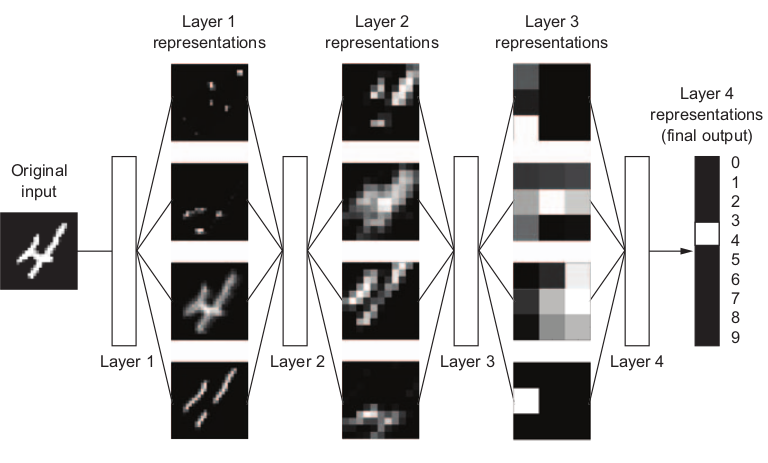
\includegraphics[width=0.8\columnwidth]{fig/digit_classification.png}
	\caption{Írott szám hozzárendelése az árbázolt számértékhez}
	\label{fig:digit_classification}
	\footnotemark
\end{figure}
\footnotetext{Forrás:\protect\cite{Chollet}}

Itt kapcsolódik össze a neurális hálózat és a mély tanulás. Az \ref{section:neuralNetworkTheory} szakaszban kifejtettem, hogy a neurális hálózat szinapszisainak paraméterezéséért felelős $W$ mátrixok és a neuronok küszöbszintjének állítására szolgáló $\vec{b}$ vektorok változóinak száma hatalamas lehet ---alkalmazástól függően több százezer, akár millió, egymástól független változóról beszélünk---, tehát beállításukhoz valamilyen algoritmusra van szükség.
Ezért a neurális hálózatok másik komponense, egy tanulási algoritmus, mely beállítja ezen paramétereket. Négy  megközelítés létezik, amikor gépi tanulásról van szó.
\emph{Ellenőrzött tanulás} során a neurális hálózatnak felcímkézett adatokat adunk meg, tehát olyan értéket rendelünk hozzájuk, amilyet szeretnénk, hogy a hálózat produkáljon. A hálózat leképezi az adatot a meghatározott reprezentációvá. A tanuló algoritmus ebből és a címkéből egy \emph{veszteség függvény} kiszámításával meghatározza, hogy mekkora az eltérés, a valamilyen értelemben vett távolság a kapott és az elvárt eredmény között. Ez alapján frissíti a $W$ mátrixokat és $\vec{b}$ vektorokat.
\emph{Ellenőrizetlen tanulás}, mely során az adatokat nem címkézzük fel, hanem arra vagyunk kíváncsiak, hogy miféle összefüggések vannak közöttük. Ezt a módszert adatbányászat során alkalmazzák. 
Az \emph{Önellenőrzött tanulás} hasonló az ellenőrzötthöz, azonban az adatok felcímkézését nem emberi erővel végezzük, hanem az adatokból állítjuk elő valamilyen heurisztikát felhasználva. Egyik alakalmazási területe az autóenkóderek tanítása.
\emph{Megerősítéses tanulás} egy újfajta megközelítése a neurális hálózatok alkalmazásának. Ennél a metodikánál a hálózatot egy ágens alkalmazza, így a hálózat bemenete az ágens által megfigyelt környezet a kimenete pedig valamilyen cselekedet, beavatkozás és tanítás során az ágens igyekszik valamilyen környezetbeli értéket maximalizálni. Gyakori alkalmazás valamilyen játékot játszó ágens, ahol azt tanulja, adott helyzetekre milyen reakcióval tudja maximalizálni játékbeli pontszmát.
Vizsgálódásomat az \emph{ellenőrzött tanulásra} korlátoztam, így a továbbiakban ennek tükrében folytatom dolgozatomat.

\section{Függvények, algoritmusok}

\subsection{Neuronok aktivációs függvényei}

\subsection{Veszteség függvények}

\subsection{,,Backpropagation'' algoritmus}

\subsection{A kernel-trükk}
